% coding:utf-8

%----------------------------------------
%FOSAMATH, a LaTeX-Code for a mathematical summary for basic analysis
%Copyright (C) 2013, Daniel Winz, Ervin Mazlagic, Adrian Imboden, Philipp Langer

%This program is free software; you can redistribute it and/or
%modify it under the terms of the GNU General Public License
%as published by the Free Software Foundation; either version 2
%of the License, or (at your option) any later version.

%This program is distributed in the hope that it will be useful,
%but WITHOUT ANY WARRANTY; without even the implied warranty of
%MERCHANTABILITY or FITNESS FOR A PARTICULAR PURPOSE.  See the
%GNU General Public License for more details.
%----------------------------------------

% coding:utf-8
\section{Darstellung von Funktionen}
\subsection{Polares Koordinatensystem}
Eine Funktion kann auch im Polaren Koordinatensystem definiert werden. 
Dabei wird jeder Punkt durch den Abstand zur Ordinate und den Winkel zur x-Achse definiert. 

\begin{figure}[h!]
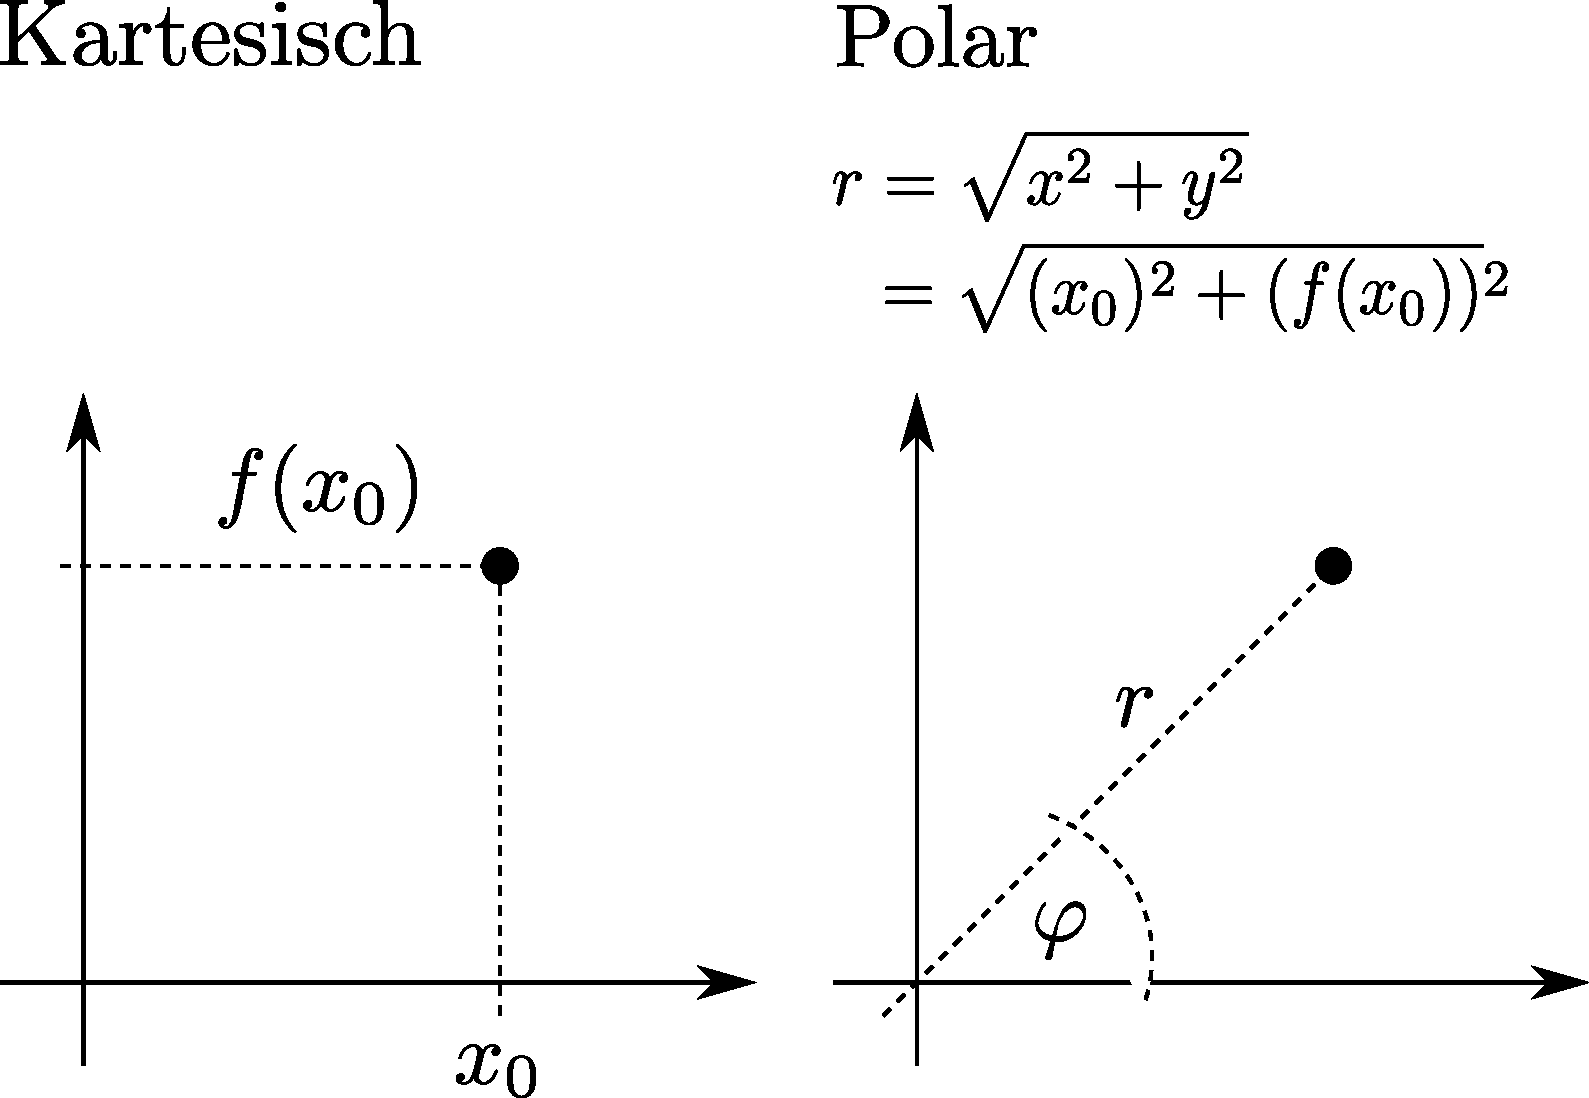
\includegraphics[width=1\textwidth]{polar.pdf}
\end{figure}

% \begin{figure}[h!]
%\includegraphics[height=1\textwidth,angle=270]{polar_2.pdf}
%\end{figure}

\subsection{Umrechnung Kartesisch $\rightarrow$ Polar}
\[ \boxed{r = \sqrt{x^2 + y^2}} \]
\[ \boxed{\varphi = \arctan\left(\frac{y}{x}\right)} \]

\subsection{Umrechnung Polar $\rightarrow$ Kartesisch}
\[ \boxed{x = r \cdot \cos{\varphi}} \]
\[ \boxed{y = r \cdot \sin{\varphi}} \]

\subsection{Parameterdarstellung}
Bei der Paramaterdarstellung wird jeder Punkt durch die x- und die y-Koordinate definiert. 
\[ \boxed{f(t) = \left(\begin{matrix} x(t)\\ y(t) \end{matrix}\right)} \] 

\noindent 
Weitere Informationen zur Ableitung in der Parameterdarstellung siehe~\ref{subsec:ableitungsregeln} (Seite \pageref{subsec:ableitungsregeln})
